\documentclass{article}
\usepackage{fullpage}
\usepackage{nopageno}
\usepackage{amsmath}
\usepackage{graphics}
\allowdisplaybreaks

\newcommand{\abs}[1]{\left\lvert #1 \right\rvert}
\newcommand{\degree}{\ensuremath{^\circ}}

\begin{document}
Jon Allen

HW 06

\begin{align*}
  \phi(x)&=\sum\limits_{n=1}^\infty{A_n\sin(n\pi x)}&A_n&=2\int_0^1{\phi(x)\sin(n\pi x)\,\mathrm{d}x}\\
  1&=\sum\limits_{n=1}^\infty{A_n\sin(n\pi x)}&A_n&=2\int_0^1{\sin(n\pi x)\,\mathrm{d}x}\\
  u&=n\pi x,\quad \mathrm{d}u=n\pi & A_n&=\frac{2}{n\pi}\int_0^1{\sin(u)\,\mathrm{d}u}\\
  A_n&=\frac{2}{n\pi}\left[-\cos u\right]_0^1=\frac{2}{n\pi}\left[-\cos(n\pi x)\right]_0^1
  &A_n&=\frac{2}{n\pi}\left[-\cos(n\pi)+\cos(0)\right]=\frac{2}{n\pi}\left(1-\cos(n\pi)\right)\\
  A_n&=\frac{2}{n\pi}\left(1-(-1)^n\right)
\end{align*}
So $A_n$ is zero for all even $n$s and $\frac{4}{n\pi}$ for odd.
\begin{align*}
  \phi(x)&=\sum\limits_{n=1}^\infty{\frac{4}{(2n-1)\pi}\sin((2n-1)\pi x)}\\
  &=\frac{4}{\pi}\left(\sin(\pi x)+\frac{1}{3}\sin(3\pi x)+\frac{1}{5}\sin(5\pi x)+\frac{1}{7}\sin(7\pi x)+\cdots\right)
\end{align*}
%\begin{figure}[tbp]
%  \begin{center}
    % GNUPLOT: LaTeX picture with Postscript
\begingroup
  \makeatletter
  \providecommand\color[2][]{%
    \GenericError{(gnuplot) \space\space\space\@spaces}{%
      Package color not loaded in conjunction with
      terminal option `colourtext'%
    }{See the gnuplot documentation for explanation.%
    }{Either use 'blacktext' in gnuplot or load the package
      color.sty in LaTeX.}%
    \renewcommand\color[2][]{}%
  }%
  \providecommand\includegraphics[2][]{%
    \GenericError{(gnuplot) \space\space\space\@spaces}{%
      Package graphicx or graphics not loaded%
    }{See the gnuplot documentation for explanation.%
    }{The gnuplot epslatex terminal needs graphicx.sty or graphics.sty.}%
    \renewcommand\includegraphics[2][]{}%
  }%
  \providecommand\rotatebox[2]{#2}%
  \@ifundefined{ifGPcolor}{%
    \newif\ifGPcolor
    \GPcolorfalse
  }{}%
  \@ifundefined{ifGPblacktext}{%
    \newif\ifGPblacktext
    \GPblacktexttrue
  }{}%
  % define a \g@addto@macro without @ in the name:
  \let\gplgaddtomacro\g@addto@macro
  % define empty templates for all commands taking text:
  \gdef\gplbacktext{}%
  \gdef\gplfronttext{}%
  \makeatother
  \ifGPblacktext
    % no textcolor at all
    \def\colorrgb#1{}%
    \def\colorgray#1{}%
  \else
    % gray or color?
    \ifGPcolor
      \def\colorrgb#1{\color[rgb]{#1}}%
      \def\colorgray#1{\color[gray]{#1}}%
      \expandafter\def\csname LTw\endcsname{\color{white}}%
      \expandafter\def\csname LTb\endcsname{\color{black}}%
      \expandafter\def\csname LTa\endcsname{\color{black}}%
      \expandafter\def\csname LT0\endcsname{\color[rgb]{1,0,0}}%
      \expandafter\def\csname LT1\endcsname{\color[rgb]{0,1,0}}%
      \expandafter\def\csname LT2\endcsname{\color[rgb]{0,0,1}}%
      \expandafter\def\csname LT3\endcsname{\color[rgb]{1,0,1}}%
      \expandafter\def\csname LT4\endcsname{\color[rgb]{0,1,1}}%
      \expandafter\def\csname LT5\endcsname{\color[rgb]{1,1,0}}%
      \expandafter\def\csname LT6\endcsname{\color[rgb]{0,0,0}}%
      \expandafter\def\csname LT7\endcsname{\color[rgb]{1,0.3,0}}%
      \expandafter\def\csname LT8\endcsname{\color[rgb]{0.5,0.5,0.5}}%
    \else
      % gray
      \def\colorrgb#1{\color{black}}%
      \def\colorgray#1{\color[gray]{#1}}%
      \expandafter\def\csname LTw\endcsname{\color{white}}%
      \expandafter\def\csname LTb\endcsname{\color{black}}%
      \expandafter\def\csname LTa\endcsname{\color{black}}%
      \expandafter\def\csname LT0\endcsname{\color{black}}%
      \expandafter\def\csname LT1\endcsname{\color{black}}%
      \expandafter\def\csname LT2\endcsname{\color{black}}%
      \expandafter\def\csname LT3\endcsname{\color{black}}%
      \expandafter\def\csname LT4\endcsname{\color{black}}%
      \expandafter\def\csname LT5\endcsname{\color{black}}%
      \expandafter\def\csname LT6\endcsname{\color{black}}%
      \expandafter\def\csname LT7\endcsname{\color{black}}%
      \expandafter\def\csname LT8\endcsname{\color{black}}%
    \fi
  \fi
  \setlength{\unitlength}{0.0500bp}%
  \begin{picture}(7200.00,5040.00)%
    \gplgaddtomacro\gplbacktext{%
      \csname LTb\endcsname%
      \put(726,440){\makebox(0,0)[r]{\strut{} 0}}%
      \put(726,1163){\makebox(0,0)[r]{\strut{} 0.2}}%
      \put(726,1885){\makebox(0,0)[r]{\strut{} 0.4}}%
      \put(726,2608){\makebox(0,0)[r]{\strut{} 0.6}}%
      \put(726,3330){\makebox(0,0)[r]{\strut{} 0.8}}%
      \put(726,4052){\makebox(0,0)[r]{\strut{} 1}}%
      \put(726,4775){\makebox(0,0)[r]{\strut{} 1.2}}%
      \put(858,220){\makebox(0,0){\strut{} 0}}%
      \put(2047,220){\makebox(0,0){\strut{} 0.2}}%
      \put(3236,220){\makebox(0,0){\strut{} 0.4}}%
      \put(4425,220){\makebox(0,0){\strut{} 0.6}}%
      \put(5614,220){\makebox(0,0){\strut{} 0.8}}%
      \put(6803,220){\makebox(0,0){\strut{} 1}}%
    }%
    \gplgaddtomacro\gplfronttext{%
      \csname LTb\endcsname%
      \put(5816,4602){\makebox(0,0)[r]{\strut{}4/pi*sin(pi*x)+4/(3*pi)*sin(3*pi*x)+4/(5*pi)*sin(5*pi*x)+4/(7*pi)*sin(7*pi*x)}}%
    }%
    \gplbacktext
    \put(0,0){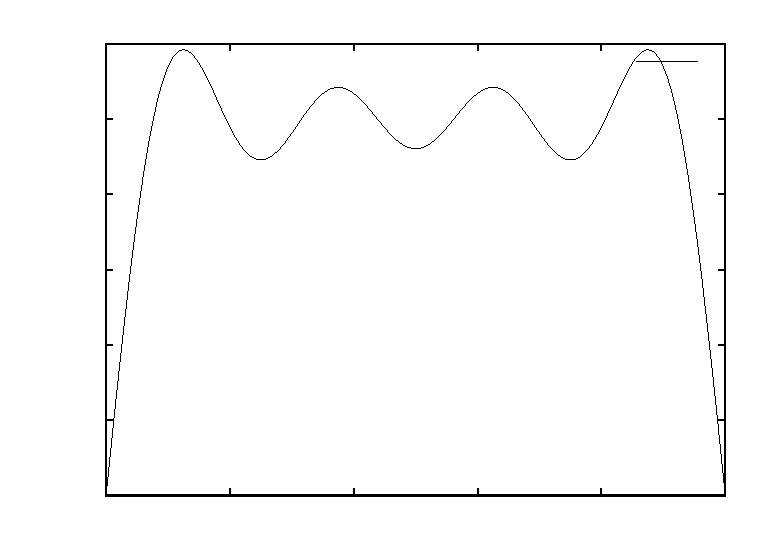
\includegraphics{pde-hw-06-plot-01}}%
    \gplfronttext
  \end{picture}%
\endgroup

%    \caption{Graph caption}
%    \label{graph:graph1}
%  \end{center}
%\end{figure}
\end{document}
